\section{Experiments and Results}

We simulate a two-dimensional SIR model with diffusion on a square domain \(\Omega = [0,L]\times [0,L]\) using a \(50\times 50\) grid.
The diffusion coefficients are set to \(\mu_S = 0.001\) and \(\mu_I = 0.001\), while the infection rate \(\beta=3.0\) is modified to be spatially and temporally dependent, as described in the previous section.

The initial conditions are chosen at random, with random positions for the infected individuals, and the simulation runs for \(T=15\).
In this case, we have an event at \(t=8\) that increases the infection rate in the top half of the domain within a certain radius.

\begin{figure}[H]
  \centering
  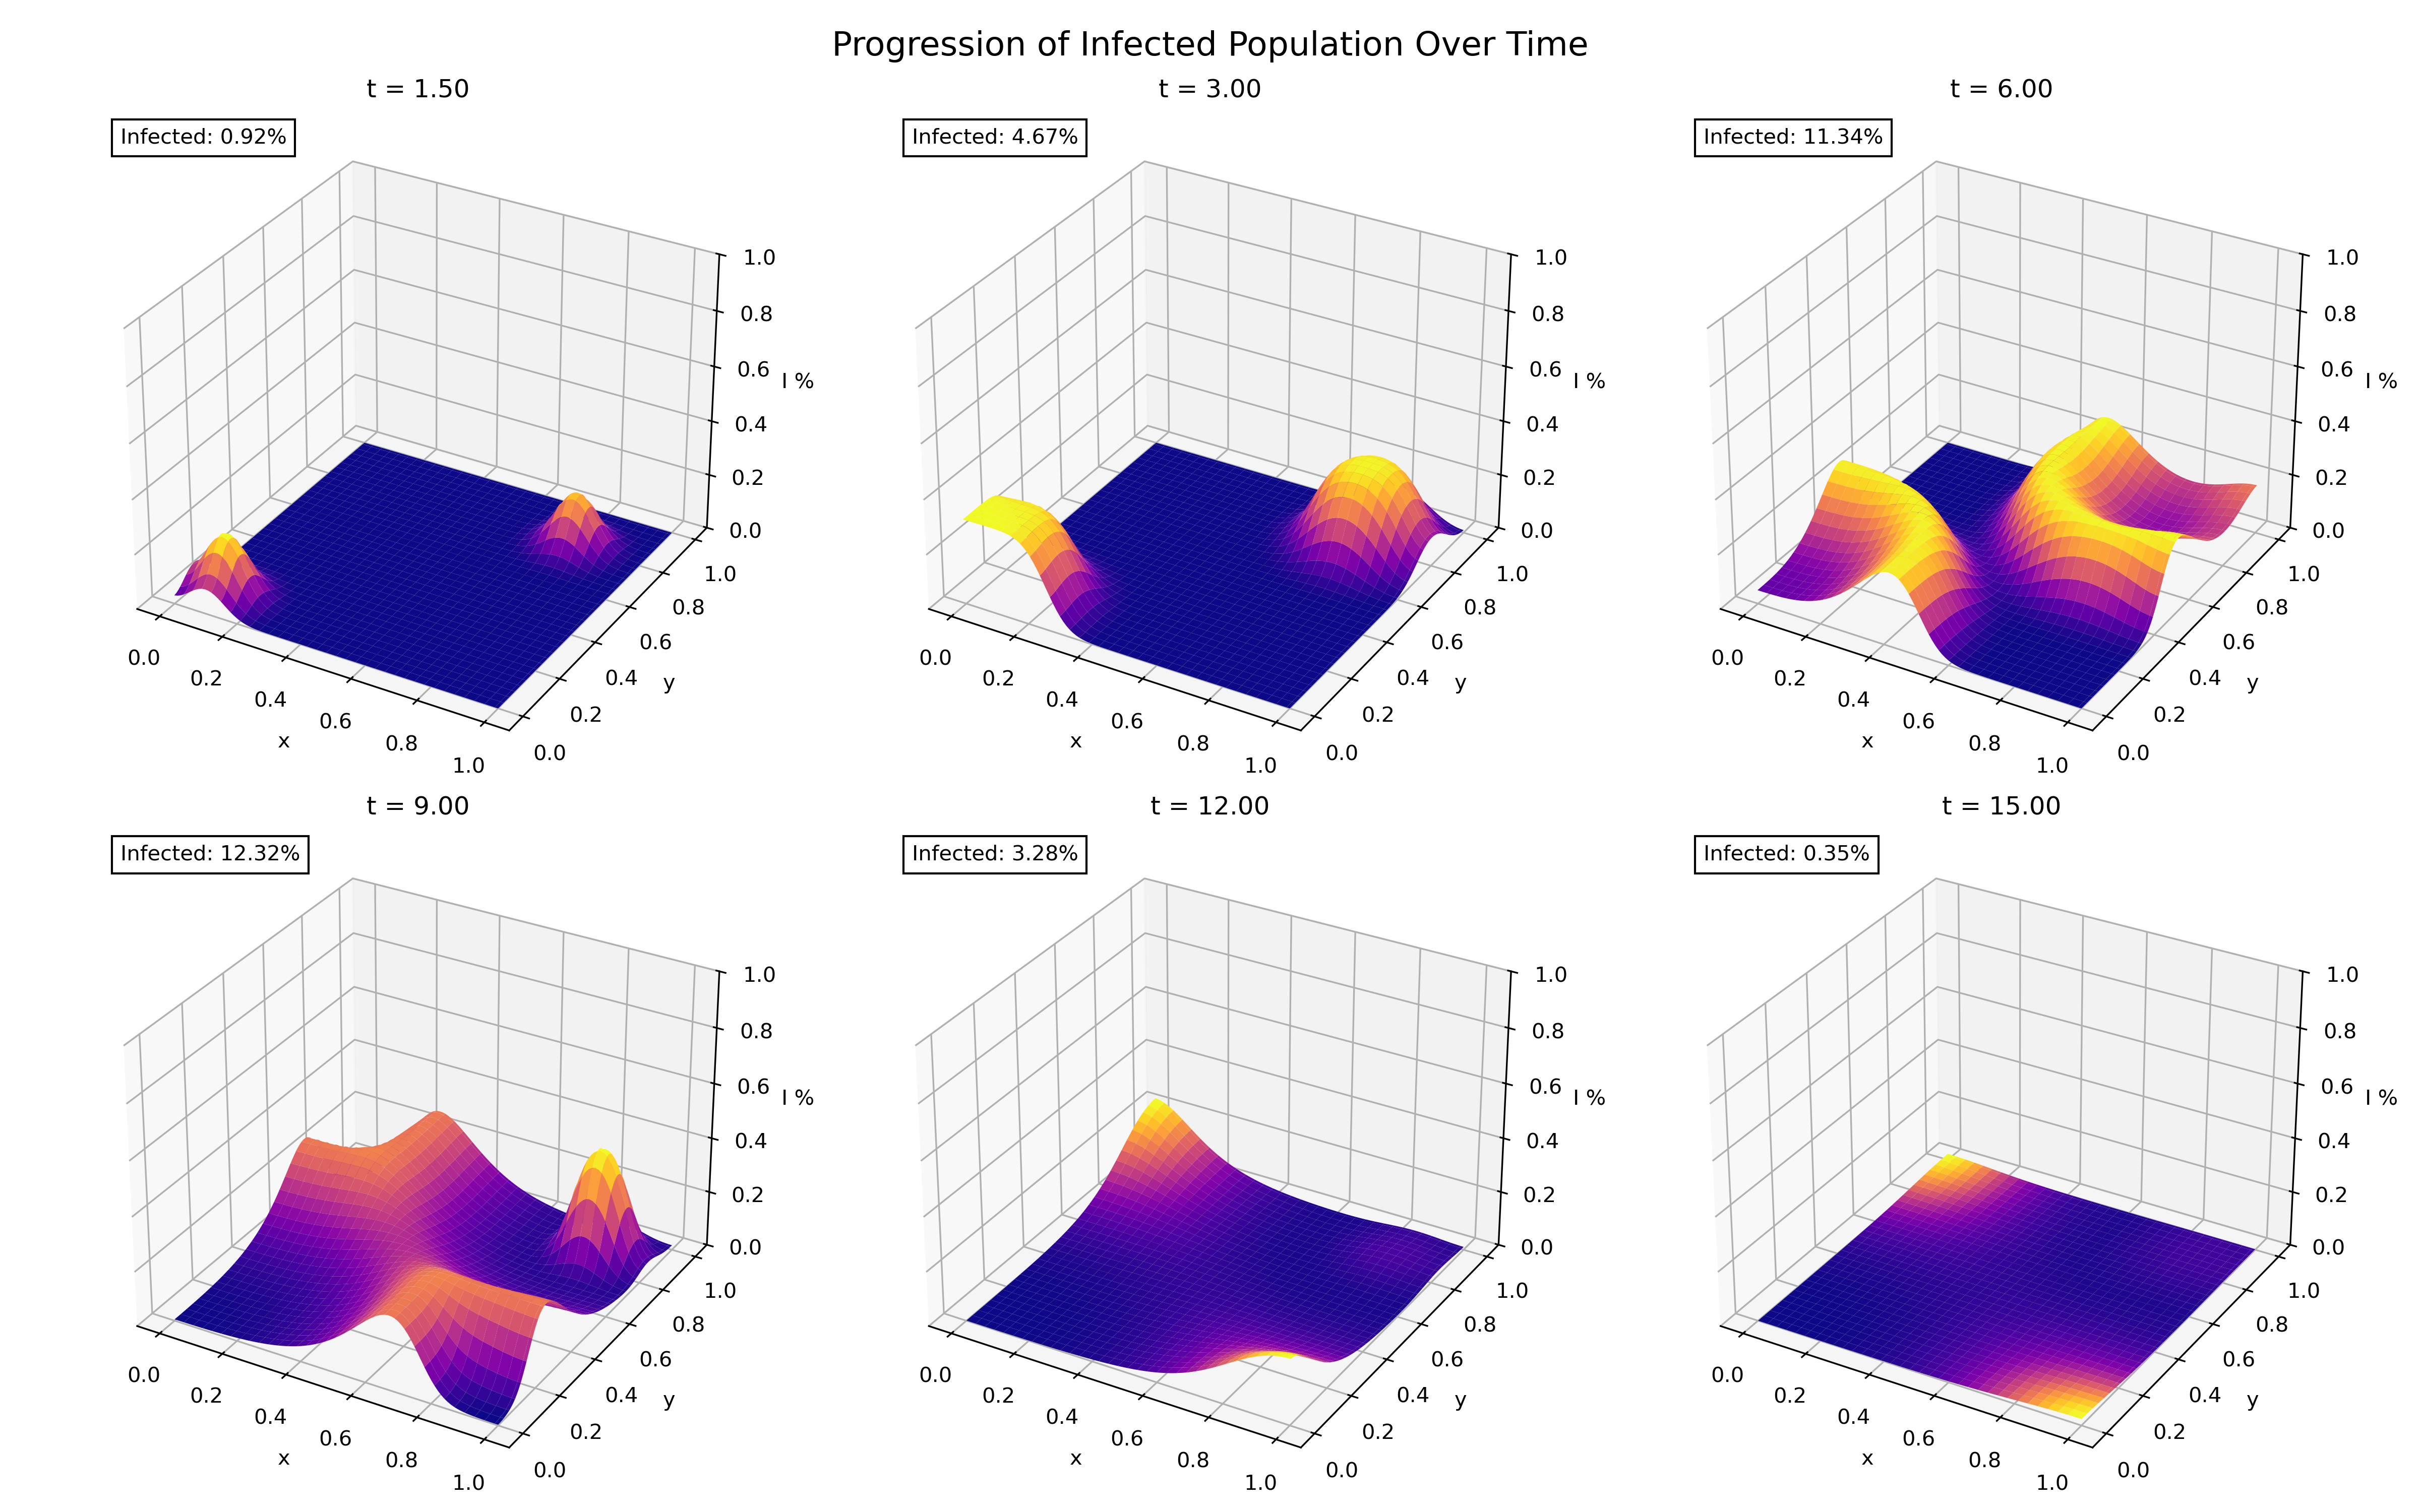
\includegraphics[width=0.5\textwidth]{figures/infected_progression.png}
  \caption{Infected population over time.}
  \label{fig:infected_progression}
\end{figure}

By combining a two-dimensional diffusion operator (for $S$ and $I$) with the usual SIR reaction terms, we capture how local infection spreads spatially. Our chosen domain and parameters illustrate various infection patterns:
\begin{itemize}
  \item \textbf{Small \(\mu_S,\mu_I\)}: keeps population mostly localized, leading to distinct infection clusters.
  \item \textbf{Modified \(\beta(x,y,t)\)}: represents spatiotemporal heterogeneity, e.g.\ higher infection rates in the central region or for certain times.
\end{itemize}
Though we used straightforward explicit Euler in time, the moderate diffusion and relatively small \(\Delta t\) suffice to maintain stability. More advanced time-stepping schemes (like Crank--Nicolson) could also be adapted for faster runs if necessary. Overall, our setup provides a flexible environment to explore how disease waves propagate and to visualize key features of spatio-temporal epidemics.